% =====================================================================
% פרק 2 — מבוא היסטורי א': משבר הסאב־פריים בארה"ב ומשבר הנדל"ן בספרד
% Owner: Agent 1. Thematic, critical literature review (guide ch.5)
% =====================================================================
\chapter{מבוא היסטורי א': משבר הסאב־פריים בארצות הברית ומשבר הנדל״ן בספרד}
\label{ch:subprime}

\begin{managerbox}
משברי \en{2008} בארה״ב ובספרד הם שני ״תסריטים״ שונים של כשל בשוק הדיור. בארה״ב הסיכון עבר מהלווים אל המערכת הפיננסית דרך איגוח ובנקאות צל. בספרד הוא הצטבר במאזני היזמים ובקופות החיסכון שמימנו אותם. מי שמנהל חשיפה לנדל״ן צריך לדעת איזה משני התסריטים קרוב יותר למצב בישראל, ופרק זה מספק את אבני הבוחן לכך.
\end{managerbox}

משבר הסאב־פריים (\en{Subprime}) של \en{2007–2009} החל כבעיית אשראי בפלח מצומצם של שוק המשכנתאות האמריקאי, והתגלגל למשבר נזילות ופירעון עולמי \cite{fcic2011,brunnermeier2009}. במקביל קרס בספרד שוק נדל״ן שנשען על תנופת בנייה ועל אשראי יזמי \cite{akin2014,bde2017}. הסקירה מאורגנת בשישה נושאים: הסכמות, מחלוקות ורלוונטיות לישראל.

\section{נושא \en{1}: היצע אשראי מול יסודות כלכליים}
\label{sec:ch2-credit}

האם עליית המחירים בארה״ב בשנים \en{1997–2006} נבעה מיסודות כלכליים או מהיצע האשראי? ריבית של \pct{1} וביקוש עולמי לנכסים ״בטוחים״ יצרו ״רעב לתשואה״ \enb{Search for Yield} \cite{brunnermeier2009}. מיאן וסופי \cite{mian2009} מצאו שאשראי המשכנתאות התרחב מהר ביותר דווקא במיקודים שבהם שיעור הלווים בדירוג נמוך היה גבוה וצמיחת ההכנסות חלשה; מכאן שהיצע האשראי, ולא היסודות, הניע את הבועה. בהמשך הראו שהפגיעה בעושר משקי הבית הממונפים הפכה את משבר הדיור למיתון הגדול \cite{mian2014}.

\paragraph{מחלוקת.} אדלינו, שואר וסברינו \cite{adelino2016} מראים שחלק גדול מהגידול באשראי ומהכשלים התרכז דווקא במעמד הביניים ובלווים בדירוג סביר. אם הסיכון אינו מוגבל ללווים ״חלשים״, גם רוכשים בהכנסה ממוצעת במבצעי \deal{20/80} עלולים להיפגע (\en{H2}).

\section{נושא \en{2}: מוצרים הדוחים את מבחן היכולת}
\label{sec:ch2-teaser}

בלב המשבר האמריקאי עמדו מוצרי משכנתא שבהם התשלום ההתחלתי היה נמוך באופן מלאכותי \cite{fcic2011}: משכנתאות טיזר מסוג \en{2/28} או \en{3/27} (\en{Teaser}, \en{ARM}), שבהן הריבית המוזלת ״התאפסה״ (\en{Reset}) לאחר שנתיים־שלוש; הלוואות \en{Interest-Only} ו־\en{Option ARM}; והלוואות \en{Low-Doc/No-Doc} ללא הוכחת הכנסה. המשותף לכולן הוא \textbf{דחיית מבחן היכולת}, כלומר מעבר ממימון גידור למימון ספקולטיבי ופונזי \cite{minsky1992}.

איור~\ref{fig:payment-shock} ממחיש את ״זעזוע התשלום״ בפרמטרים מכוילים. בתרחיש להמחשה, הלוואה של \en{\$200,000} שעברה מריבית של \pct{8} ל־\pct{11} העלתה את ההחזר החודשי ב־\pct{29} ואת יחס ההחזר מ־\pct{40} ל־\pct{51.5}. בעסקאות \deal{20/80} ו־\deal{20/50/30} הקפיצה ביום המסירה חדה יותר: מאפס, או מ־\pct{20.5} בתשלום ריבית בלבד, ל־\pct{36} מההכנסה.

\begin{figure}[!htb]
\centering
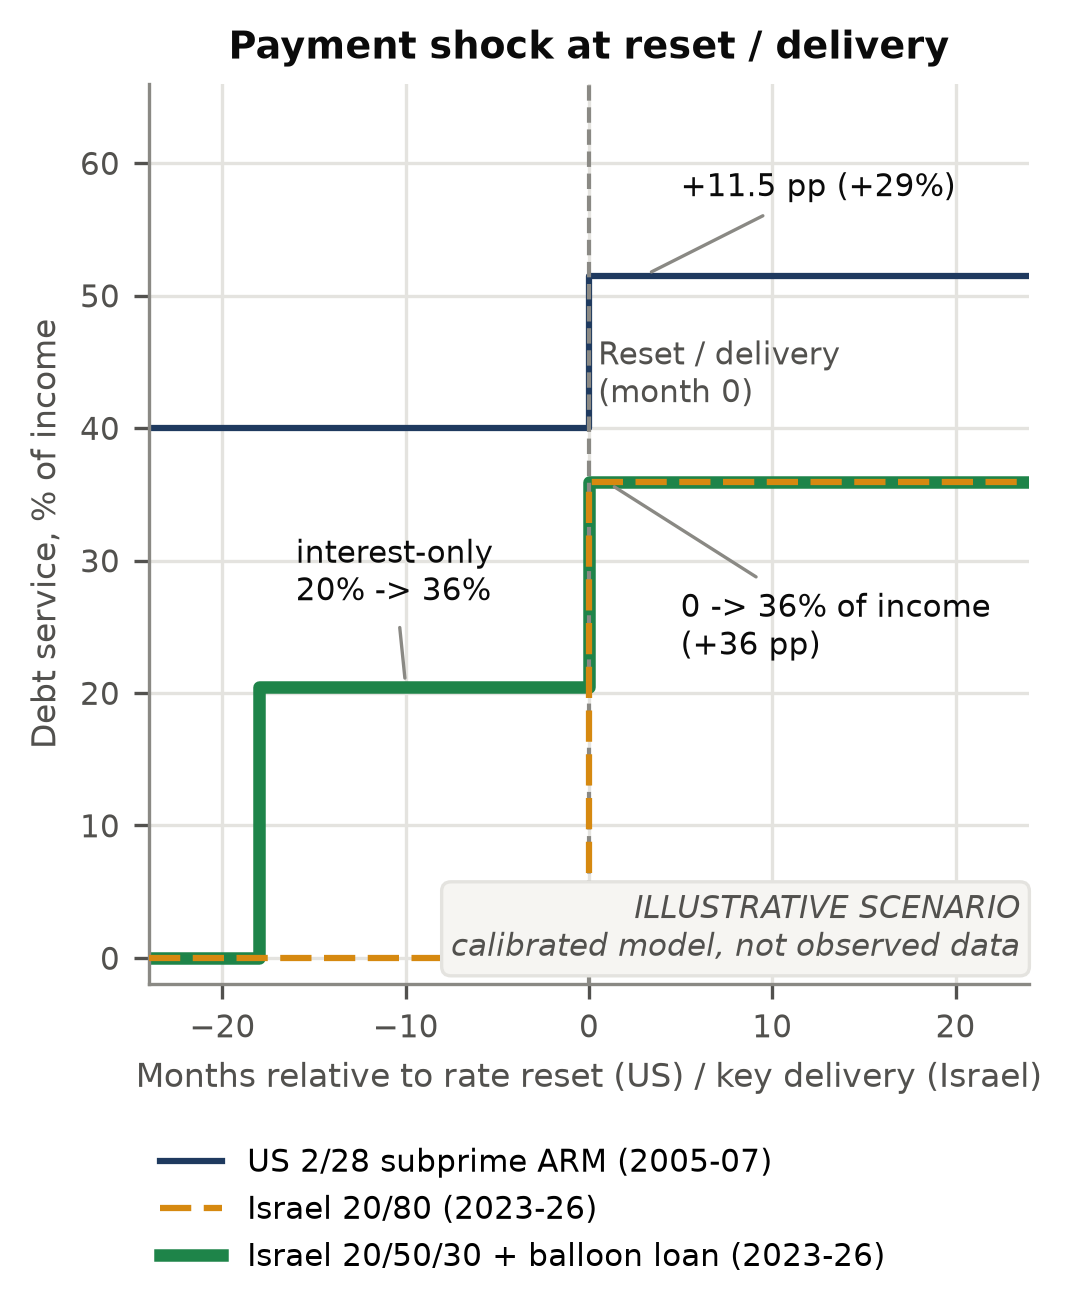
\includegraphics[width=0.62\textwidth]{figures/fig1_payment_shock_2080_vs_teaser.png}
\caption[זעזוע התשלום בנקודת האיפוס: טיזר \en{2/28} מול \en{20/80} ו־\en{20/50/30}]{זעזוע התשלום בנקודת האיפוס: משכנתת טיזר \en{2/28} בארה״ב (\en{2005–2007}) לעומת עסקאות \en{20/80} ו־\en{20/50/30} בישראל, כשיעור מהכנסת משק הבית. תרחיש להמחשה בפרמטרים מכוילים (פרק~\ref{ch:methodology})}
\label{fig:payment-shock}
\end{figure}

\section{נושא \en{3}: איגוח, דירוג וסיכון מוסרי}
\label{sec:ch2-securitization}

\sloppy מבנה התמריצים השתנה במעבר ממודל ״הפקה לשם החזקה״ \enb{Originate-to-Hold} למודל ״הפקה לשם הפצה״ \enb{Originate-to-Distribute}. מלווים, חלקם ללא פיקוח בנקאי, מכרו הלוואות לבנקי השקעות, שאיגדו אותן ל\term{ניירות ערך מגובי משכנתאות}{MBS} ואיגדו מחדש את שכבות הביניים ל\term{אגרות חוב מובטחות בחוב}{CDO}. קיז ושותפיו \cite{keys2010} מצאו שהאיגוח הוביל לסינון רשלני יותר של לווים, כתחזית תאוריית הסיכון המוסרי, ו־\pct{83} מניירות הערך שדירגה \en{Moody's} בדירוג \en{AAA} בשנת \en{2006} הורדו לבסוף בדירוגם \cite{fcic2011}. \textbf{רלוונטיות לישראל:} בישראל חקיקת האיגוח טרם הושלמה \cite{boi_survey2025,hapoalim_q3_2026}, ונראה שערוץ ההעברה המרכזי של המשבר האמריקאי אינו קיים בהיקף דומה (\en{H3}). מנגד, ההיגיון של ״מוכר שאינו נושא בסיכון״ חוזר בצורה אחרת: היזם מקבל תמורה מוקדמת, ומבחן היכולת של הרוכש נדחה.\par\fussy

\section{נושא \en{4}: בנקאות צל וריצה על הנזילות}
\label{sec:ch2-shadow}

חלק ניכר מהנכסים המאוגחים הוחזק בגופים מחוץ למאזן הבנקים (\en{SIVs}, \en{Conduits}), שמומנו בנייר ערך מסחרי קצר מועד ובהסכמי רכש חוזר (\en{Repo}). פוזסר ושותפיו \cite{pozsar2010} מעריכים שערב המשבר עלו התחייבויות מערכת הצל האמריקאית על אלה של המערכת הבנקאית המסורתית. גורטון ומטריק \cite{gorton2012} מתארים כיצד העלאת שיעורי הביטחון (\en{Haircuts}) בשוק הריפו יצרה ״ריצה״ מודרנית. \textbf{רלוונטיות לישראל:} אשראי חוץ־בנקאי ליזמים ומימון ריבית ישיר בידי היזם הם המקבילה הישראלית ל״צל״: ערוצים שהפיקוח על הבנקים אינו מגביל ישירות (\en{H1}).

\section{נושא \en{5}: עיקולים, חבות אישית והלולאה ההרסנית}
\label{sec:ch2-foreclosures}

העלאת הריבית בארה״ב מ־\pct{1} ל־\pct{5.25} (\en{2004–2006}), יחד עם מועדי האיפוס ובלימת עליית המחירים, חסמה את המימון מחדש, ושיעורי הפיגור זינקו. בחלק ממדינות ארה״ב נהגו הלוואות ״ללא חבות אישית״ \enb{Non-Recourse}, ולווה בהון עצמי שלילי \enb{Negative Equity} יכול היה למסור את המפתחות ולהשתחרר מהחוב: ״פירעון אסטרטגי״ \enb{Strategic Default}. כארבעה מיליון משפחות איבדו את בתיהן בעיקול, ומכירות העיקולים הורידו מחירים והעמיקו את הלולאה \cite{fcic2011}. \textbf{רלוונטיות לישראל:} המשכנתאות בישראל הן בחבות אישית מלאה \enb{Full Recourse}, ולכן התמריץ לפירעון אסטרטגי נמוך. מנגד, לרוכש במבצע \deal{20/80} שטרם נטל משכנתא עשויה להיות דרך יציאה אחרת, ביטול החוזה מול היזם, והסיכון עובר אז ליזם (\en{H3}).

\section{נושא \en{6}: ספרד — מלאי, יזמים ואשראי מרוכז}
\label{sec:ch2-spain}

במרכז משבר הנדל״ן הספרדי (\en{2008–2013}) עמדו היזמים (\en{Promotores}) והמלאי הלא־מכור, ולא מכשירים מאוגחים. בתנופת הבנייה של \en{1997–2007} הוזרם האשראי לבינוי ולנדל״ן במידה רבה דרך קופות החיסכון האזוריות \enb{Cajas de Ahorros}, שהיו נתונות להשפעה פוליטית ולממשל תאגידי חלש \cite{akin2014,bde2017}. עם פרוץ המשבר נעצרו המכירות, יזמים רבים קרסו, והאשראי לקרקעות ולבנייה הפך לנכסים בעייתיים, שהועברו בשנת \en{2012}, במסגרת סיוע אירופי, לחברת \en{SAREB} \cite{bde2017}.

\paragraph{מחלוקת: האם רגולציה מאקרו־יציבותית מספיקה?} חימנס ושותפיו \cite{jimenez2017} מראים שההפרשות הדינמיות האנטי־מחזוריות של ספרד ריככו את קיצוץ האשראי בשפל, אך לא מנעו את הבועה ולא את הצורך בחילוץ. הלקח לישראל: מגבלות \en{LTV/PTI} ודרישות הון אינן מבטיחות לבדן חסינות אם הבנקים חשופים במידה מופרזת לאשראי יזמי (\en{H3}).

\section{מטריצת הספרות וסינתזה}
\label{sec:ch2-matrix}

מטבלה~\ref{tab:ch2-matrix}, הממפה את המקורות לנושאים, עולות שתי תובנות: נושאי האשראי והאיגוח (\en{T1}, \en{T3}) נחקרו בהרחבה, ואילו הצד היזמי (\en{T6}) נחקר מעט ובעיקר בהקשר הספרדי; ואף מקור אינו בוחן מוצר שבו \textbf{היזם} הוא שדוחה את מבחן היכולת של הרוכש, וזהו המאפיין הייחודי של השוק הישראלי. לשני המשברים ליבה משותפת \cite{reinhart2009}: מנגנוני המינוף לובשים צורה חדשה בכל מחזור, אך המהות חוזרת, דחיית ההכרה בסיכון והישענות על המשך עליית המחירים. טבלה~\ref{tab:ch2-mechanisms} מתרגמת את מנגנוני הכשל להקבלות אפשריות בישראל ולהשערה הבוחנת כל אחת מהן.

\begin{table}[!htb]
\centering
\caption{מטריצת ספרות: מקורות מרכזיים מול נושאי הסקירה}
\label{tab:ch2-matrix}
\footnotesize
\begin{tabularx}{\tabmaxwidth}{>{\raggedleft\arraybackslash}p{5.2cm} C C C C C C}
\toprule
\hd{מקור} & \hd{\en{T1}} & \hd{\en{T2}} & \hd{\en{T3}} & \hd{\en{T4}} & \hd{\en{T5}} & \hd{\en{T6}} \\
\midrule
\en{Minsky (1986; 1992)} \cite{minsky1986,minsky1992} & $\bullet$ & $\bullet$ & & & & $\bullet$ \\
\en{Akerlof (1970)} \cite{akerlof1970} & & & $\bullet$ & & & \\
\en{Stiglitz \& Weiss (1981)} \cite{stiglitz1981} & $\bullet$ & & $\bullet$ & & & \\
\en{Reinhart \& Rogoff (2009)} \cite{reinhart2009} & $\bullet$ & & & & $\bullet$ & $\bullet$ \\
\en{Brunnermeier (2009)} \cite{brunnermeier2009} & $\bullet$ & & $\bullet$ & $\bullet$ & & \\
\en{Mian \& Sufi (2009)} \cite{mian2009} & $\bullet$ & $\bullet$ & & & $\bullet$ & \\
\en{Keys et al. (2010)} \cite{keys2010} & & & $\bullet$ & & & \\
\en{Pozsar et al. (2010)} \cite{pozsar2010} & & & $\bullet$ & $\bullet$ & & \\
\en{FCIC (2011)} \cite{fcic2011} & $\bullet$ & $\bullet$ & $\bullet$ & $\bullet$ & $\bullet$ & \\
\en{Gorton \& Metrick (2012)} \cite{gorton2012} & & & $\bullet$ & $\bullet$ & & \\
\en{Akin et al. (2014)} \cite{akin2014} & $\bullet$ & & & & & $\bullet$ \\
\en{Mian \& Sufi (2014)} \cite{mian2014} & $\bullet$ & & & & $\bullet$ & \\
\en{Shiller (2015)} \cite{shiller2015} & $\bullet$ & & & & & \\
\en{Adelino et al. (2016)} \cite{adelino2016} & $\bullet$ & $\bullet$ & & & $\bullet$ & \\
\en{Jiménez et al. (2017)} \cite{jimenez2017} & $\bullet$ & & & & & $\bullet$ \\
\en{Banco de España (2017)} \cite{bde2017} & & & & & $\bullet$ & $\bullet$ \\
\bottomrule
\multicolumn{7}{p{12cm}}{\scriptsize \en{T1}: היצע אשראי מול יסודות; \en{T2}: דחיית מבחן היכולת; \en{T3}: איגוח, דירוג וסיכון מוסרי; \en{T4}: בנקאות צל ונזילות; \en{T5}: עיקולים וחבות; \en{T6}: יזמים, מלאי ואשראי מרוכז.} \\
\end{tabularx}
\vspace{0.8em}
\caption{מנגנוני כשל במשברי \en{2008} והקבלתם האפשרית לשוק הישראלי}
\label{tab:ch2-mechanisms}
\footnotesize
\begin{tabularx}{\tabmaxwidth}{R R R >{\centering\arraybackslash}p{1.3cm}}
\toprule
\hd{מנגנון כשל} & \hd{ארה״ב / ספרד} & \hd{מקבילה אפשרית בישראל} & \hd{השערה} \\
\midrule
דחיית מבחן היכולת & \en{Teaser/ARM}, \en{Interest-Only} & \deal{20/80}, \deal{20/50/30}, הלוואות בלון & \en{H1, H2} \\
\midrule
אשראי מחוץ לפיקוח & בנקאות צל, ריפו & מימון ריבית בידי היזם, אשראי חוץ־בנקאי & \en{H1} \\
\midrule
הסתרת המחיר האמיתי & דירוגים מנופחים & מחיר מחירון מול \en{NPV} כלכלי & \en{H1} \\
\midrule
זעזוע ריבית במועד האיפוס & איפוס ריבית \en{2006–2007} & משכנתא בריבית גבוהה במסירה & \en{H2} \\
\midrule
מלאי וקריסת יזמים & ספרד: \en{Promotores}, \en{Cajas} & מלאי של למעלה מ־\en{85,000} דירות & \en{H3} \\
\midrule
העברת הסיכון לבנקים & \en{Non-Recourse}, איגוח & ליווי סגור, חוק המכר, \en{Full Recourse} & \en{H3} \\
\bottomrule
\end{tabularx}
\end{table}

לאחר שזוהו מנגנוני הכשל של \en{2008}, הפרק הבא בוחן כיצד התפתח שוק הדיור הישראלי בשנים \en{2022–2026}, ואילו מן המנגנונים הללו ניכרים בו.
